
\cleartoverso 
\chaptercontents{Homological Algebra}{homologicalcover.tex}{These notes are meant as a quick reference guide for the constructions in homological algebra that we will use throughout the course, and are not in any way suppose to be a substitute for a proper set of notes on homological algebra.}
\label{chap:homologicalalgebra}

\begin{elevator}[An introduction to Chain Complexes]
	A short introduction to chain complexes.
\end{elevator}

\label{sec:chaincomplexes:intro}
\subsection{Vector Spaces, Sets, Diagrams and Notations}
Before we start with the development of homological algebra, it is a good idea to set up some common conventions for doing abstract linear algebra diagrammatically. We've already developed some of these tools independently in \ref{sec:graph:cyclespace}, but we should flush out these methods more fully before proceeding to develop chain complexes. \\
\begin{definition}
Let $V_1, V_2$ be two vector spaces. The \emph{direct sum} of $V_1$ and $V_2$ is the vector space of pairs of vectors between them, and is denoted 
\[V_1\oplus V_2:=\{(v_1, v_2)\;|\; v_1\in V_1, v_2\in V_2\}.\]
\end{definition}
\begin{example}
The set of $n$-tuples of real numbers is usually denoted $\RR^n$. Another way of presenting this vector space is 
\[\RR^n=\underbrace{\RR\oplus \RR \oplus \cdots \oplus \RR\oplus \RR}_n\]
where now each ``vector'' $r_i\in R^1_i$ is a scalar. 
\end{example}
\begin{example}The rank nullity theorem can be restated that if $f: V\to W$ is a map, then 
\[V\simeq \ker f\oplus \im f. \]
\end{example}
Given vector spaces $V_1, V_2, W$, and maps $f_1: V_1\to W$, $f_2: V_2\to W$, one can create a new map from $V_1\oplus V_2\to W$, which is defined by taking the sum of the two maps:
\begin{align*}
f_1\oplus f_2: V_1\oplus V_2 \to&  W\\
(v_1, v_2)\mapsto f_1(v_1)+f_2(v_2).
\end{align*}
We will frequently represent this composition either \emph{diagrammatically} or {using matrices.} The diagrammatic presentation of the direct sum of maps is:
\[
\begin{tikzcd}
V_1\arrow{dr}{f_1}\\
\oplus & W\\
V_2 \arrow{ur}{f_2}
\end{tikzcd}.
\]
This is a useful shorthand, and we will use it throughout this section on chain complexes. \\
If we want to think of the direct sum as a matrix we will write it at 
\[\begin{pmatrix} f_1 & f_2 \end{pmatrix} \cdot \begin{pmatrix} v_1\\v_2\end{pmatrix} = \begin{pmatrix}f_1(v_1)+f_2(v_2) \end{pmatrix}.\]
There is nothing that limits us to taking the direct sum of more than one map along the domain. 
\begin{definition}
Let $f_i: V_i\to W$ be a collection of maps. Then define $\bigoplus_{i=1}^k f_i: \bigoplus_{i=1}^k V_i\to W$ be the map defined on tuples by
\[\left(\bigoplus f_i\right)(v_1, \ldots, v_{k})=\sum_{i=1}^k f_i(v_i).\]
\end{definition}
Similarly, this map can be represented diagrammatically. \\
Just as we can take the sum along the domains of maps, we are allowed to take sums along the codomains of maps. Let $g_1: V\to W_1$ and $g_2: V\to W_2$ be two linear maps. Then denote the direct sum along the codomain
\begin{align*}
g_1\oplus g_2: V\to & W_1\oplus W_2\\
v\mapsto (g_1(v), g_2(v).)
\end{align*}
Just as we did for direct sum along the domain, we can represent these maps diagrammatically or with matrices. 
\[\begin{tikzcd}
\;& W_1\\
V\arrow{ur}{g_1}   \arrow{dr}{g_2} & \oplus \\
\; & W_2 
\end{tikzcd}\;\;\;\;\;\;\;\;\;\;\;\;\begin{pmatrix} g_1 \\ g_2 \end{pmatrix} \cdot \begin{pmatrix} v\end{pmatrix} = \begin{pmatrix}g_1(v_1)\\g_2(v_2) \end{pmatrix}.\]
We can quickly do this with many codomains at the same time.
\begin{definition}
Let $g_i: V\to W_i$ be a collection of linear maps. Define their direct sum to be 
\begin{align*}
\bigoplus_{i=1}^k g_i: V\to& \bigoplus_{i=1}^k W_i\\
v\mapsto &(g_1(v), g_2(v) \cdots , g_k(v)).
\end{align*}
\end{definition}
By combining both processes, we can create maps from many domains and codomains simultaneously. 
\begin{definition}
Let $f_{ij}: V_i\to W_j$ be a collection of linear maps. Define their direct sum to be 
\begin{align*}
\bigoplus_{i,j} f_{ij}: \bigoplus_{i=1}^m V_i\to\bigoplus_{j=1}^n\\
(v_1, \ldots, v_m)\mapsto & \left(\sum_{i=1}^mf_{i,1}(v_i), \sum_{i=1}^mf_{i,2}(v_i), \ldots, \sum_{i=1}^mf_{i,{n-1}}(v_i), \sum_{i=1}^mf_{i,{n}}(v_i)\right).
\end{align*}
\end{definition}
We again have diagrammatic and matrix notations for these maps. 
\[
\begin{tikzcd}[row sep= tiny]
V_1\arrow{r} \arrow{rdd}  & W_1\\
\oplus & \oplus \\
V_2\arrow{r}  \arrow{ruu} & W_2
\end{tikzcd}\;\;\;\;\;\;\;\;\;\;\;\;
\begin{pmatrix}
f_{11}& f_{21}\\f_{12} & f_{22}
\end{pmatrix}
\begin{pmatrix} v_1 \\ v_2\end{pmatrix} = \begin{pmatrix} f_{11})(v_1)+f_{21}(v_2)\\ f_{12}(v_1)+f_{22}(v_2)\end{pmatrix}.
\]


\subsection{Chain Complexes, Homology, and Chain Maps}
Homological Algebra is a algebraic tool that we'll return to at several points throughout the course, and it makes sense to combine the general facts of the theory in one place. 
\begin{definition}  A \emph{chain complex} is a sequence of vector spaces, $\ldots C_{-1},C_{0},C_{1}\ldots$ and boundary maps $\partial_n:C_n\to C_{n-1}$ with the condition that $$\partial_{n-1}\circ \partial_{n}=0.$$ Frequently, we represent a chain complex with the following diagram of vector spaces and maps: $$
\begin{tikzcd}
    \cdots\arrow{r}{\partial_{2}}&    C_{1}\arrow{r}{\partial_{1}} &C_{0} \arrow{r}{\partial_0}  &C_{-1}\arrow{r}{\partial_{-1}}&\cdots \\
\end{tikzcd}$$ We will usually denote the chain complex as $( C_\bullet, \partial_\bullet)$, where $C_\bullet$ is the sequence of modules and $\partial_\bullet$ the sequence of boundary maps.\footnote{There is no particular reason for the numbers to decrease. We could make the numbers increase, and we would call it \emph{cohomology} instead.} \label{def:chaincomplex}
\end{definition}
\nomenclature{$(C, \partial)$}{A chain complex}
\begin{projectdescription}{Foo}
In principle, all of the tools that we are developing with chain complexes can be defined with rings and modules instead of just vector spaces. In fact, the field of homological algebra generally works \label{proj:abelian} over any  \emph{Abelian category,} which is a category equipped ith the necessary structures to make linear algebra-like constructions. 
\end{projectdescription}
\begin{example}
Let's look at a first example of a chain complex. Let $C_1=C_2= C_3=\RR^2$, so that we may represent our boundary maps by matrices. Consider the sequence of maps 
\[
\begin{tikzcd}[ampersand replacement=\&, column sep= large] 
0 \arrow{r}{0} \& \RR^2 \arrow{r}{\begin{pmatrix}1&0\\0&0\end{pmatrix}} \& \RR^2 \arrow{r}{\begin{pmatrix}0&0\\0&1\end{pmatrix}} \& \RR^2 \arrow{r}{0} \& 0 
\end{tikzcd}
\]
This is an example of a chain complex, as the composition of the differential is zero:
\[\partial_2\circ \partial_3 = \begin{pmatrix}0&0\\0&1\end{pmatrix}\cdot \begin{pmatrix}1&0\\0&0\end{pmatrix}=\begin{pmatrix} 0&0\\0&0\end{pmatrix}.\]
\end{example}
The boundary squaring to zero is equivalent to the statement that the image of the boundary map $\partial_{k+1}$ is in the kernel of the map $\partial_{k}$.\\
The theory of homology was developed and inspired from techniques in topology, but it is a very useful algebraic framework to have in mind. Abstractly, the chain complexes and homology are a tool that explains the relations, and relations of relations, and higher meta-relations. For example, Let $V$ be a set with a relation $E\subset V\times V$ on it. Let $\mathcal V, \mathcal E$ be the vector spaces which have $V$ and $E$ as basis respectively. One might state the relationship now in terms of a map $\partial: \mathcal E \to \mathcal V$, whose image tells us if 2 points in $V$ are related. \\
However, the framework of homology allows us to put relations on the set of relations, by introducing maps $\mathcal F\to \mathcal E$, and so on. \\
 We have seen multiple examples of chain complexes throughout this course. 
The above example is more than just a chain complex; it is \emph{exact} in that $\ker\partial_k=\im\partial_{k+1}.$ We'll explore exact complexes in more detail in the future. 
\begin{example}[Graph Complex]
A simple example of a chain complex comes from our exploration of graph theory. The edge space, vertex space, and boundary map from Definition \ref{def:graphcomplex} is an example of a chain complex, albeit a very short one. Two points $v, w$ have the property that their sum is in the image of $\partial: \mathcal E\to \mathcal V$ if there is a path $P\in\mathcal E$ between them. In this case, $\partial(P)=v+w$. 
\end{example}
\begin{example}[Embedded Graph Complex]
Recall, if we have a net $G$ for a surface $\Sigma$, we get an associated chain complex in Definition \ref{def:surfacecomplex}. This chain complex can be modified to capture the full topological data of $\Sigma$. In a way similar to the graph complex, vertices are related if there exists a path between them. However, in this example, we have a higher relation: paths are related if there exists a subsurface which has that path as it's boundary. 
\end{example}
\begin{example}[Simplicial Homology]
The Chain complex associated to a simplicial complex \ref{def:simplicialhomology} is the natural generalization of the previous two constructions. The elements of this chain complex are $k$-dimensional sub-complexes, and two subcomplexes are related if they are the boundary components of a common $k+1$ dimensional subcomplex.
\end{example}
While the examples that we've looked at in class are inspired from topology, there are many examples come from different branches of mathematics. 
\begin{definition} Let $(C,\partial_\bullet)$ be a chain complex The \emph{homology} of $\C$ at $n$ is defined to be the module 
\[H_n(C)=\frac{\ker \partial_n}{ \im \partial_{n+1}}\]
 As the composition $\partial_n \partial_{n+1}=0$, this is well defined.
 \label{def:homologygroups}
\end{definition}
\nomenclature{$H_k(C)$}{The $k$-th homology group of $(C, \partial)$}
For convenience, we will often call the kernel of $\partial_{n}$ the set of cycles, and write it $Z_n$. The image of $\partial_{n+1}$ is the set of boundaries and will be written $B_n$. Then $H_n(C)=Z_n/B_n$. The names cycles and boundaries correspond to the geometric interpretation of the homology as given above.  
\begin{definition} We say that a chain complex is \emph{bounded} if there exists $n$ such that $C_i=0$ if $|i|\geq n$.
\end{definition}
While it doesn't make sense to ask about the dimension of a chain complex, there is a generalization of dimension which applies to chain complexes. 
\begin{definition}
Let $(C, \partial)$ be a bounded chain complex  with each $C_i$ of finite dimension. Then the \emph{Euler Characteristic} of $(C, \partial)$ is the integer 
\[\chi(C, \partial):= \sum_{k=-\infty}^\infty (-1)^k \dim (C_k).\]
\end{definition}
Notice that the Euler Characteristic has no dependence on the differential of a chain complex. However, it is intimately related to the chain structure through an application of the rank-nullity theorem.  
\nomenclature{$\chi(C, \partial)$}{The Euler Characteristic of a Chain Complex}
\begin{lemma}[Euler Characteristic] Suppose that the chain complex is bounded. Then $$\chi(C, \partial) =\sum_{k=-\infty}^\infty -1^k \dim H_k.$$ 
\label{lemma:eulercharacteristic}
\end{lemma}
\begin{proof} Because our complex is bounded, there exists $n$ such that $|k|\geq n$ implies that $C_k=H_k=0$. Then we proceed by computing the sum:
\begin{align*}
\chi(C, \partial)=&\sum_{k=-i}^{i}(-1)^k C_k\\
\intertext{Applying the Rank-Nullity theorem}
 &=\sum_{k=-i}^{i}(-1)^k (\dim (\ker \partial_k )+\dim( \im \partial_k))\\
 \intertext{Shifting the sum}
 &=\sum_{k=-i}^{i}(-1)^k \dim(\ker \partial_k)-\sum_{k=-i}^{i}(-1)^{k-1} \dim( \im \partial_k)\\
 &=\sum_{k=-i}^{i}(-1)^k \dim( \ker \partial_k) - \dim (\im \partial_{k+1})\\&= \sum_{k=-i}^{i}-1^k \dim H_k\end{align*}
\end{proof}

Now that we have chain complexes, we want to look at functions that can go between them. Just like when we study vector spaces and groups, it is only useful to study the maps between these objects which preserve their structure, We want the function between chain complexes to be compatible with the differential.
\begin{definition}[Chain map] \label{def:chainmap} Let $( A,\partial^A)$ and $( B, \partial^B)$ be chain complexes, and let $f_i:A_i\to B_i$ be a collection of maps. Then we say that $f_\bullet=\{f_i\}$ is a \emph{chain map} if the following diagram commutes for all $i$:
\[\begin{tikzcd}A_i\arrow{r}{\partial_i^A}\arrow{d}{f_i}&A_{i-1}\arrow{d}{f_{i-1}}\\ B_i\arrow{r}{\partial_i^B} &B_{i-1} 
\end{tikzcd}\] \end{definition} 
A chain map not only preserves the boundary structure of the chain complex, it also gives us maps between their homology groups. 
\begin{claim}
Let $f_\bullet:(A, \partial^A)\to (B, \partial^B)$ be a chain map. Then there is a well defined map between the homology of $(A, \partial^A)$ and $(B, \partial^B)$ given by 
\begin{align*}
(f_k)_*: H_k(A)\to& H_k(B)\\
[a]\mapsto& [f_k(a)]. 
\end{align*}
\end{claim}
\begin{proof}
In order to show that this map is well defined, we need to check two things.  First we must show  that elements representing homology classes in $A$ get sent to elements representing homology classes in $B$ . Second, we must show that resulting map does not depend on the choice of representative for $a$. 
\begin{itemize}
\item For the first part, let $[a]\in H_k(A)$ be an element of homology. In order for $[f_k(a)]$ to be an element of $H_k(B)$, we need that $f_k(a)\in \ker \partial^B.$ We make a computation:
\begin{align*}
\partial^B(f_k(a))=& f_k(\partial^A(a))
\intertext{Since $[a]\in H_k(A)$, we know that $a\in \ker \partial^A$. }
=& f_k(0)=0. 
\end{align*}
\item For the second part, suppose we have 2 different representatives of the same homology class $[a]=[a']\in H_k(A)$. We would like to show that $[f_k(a)]=[f_k(a')]\in H_k(B)$. \\
Two classes in homology are equivalent if they differ by a boundary. This means we need to find $\beta$ so that  
\[[f_k(a)]-[f_k(a')]=\partial_{k+1}(\beta)\]
We can construct this $\beta$ by looking at the difference $a-a'.$  Since $[a]=[a']$, there is an element $\alpha\in C_{k+1}(A)$ so that $\partial^A(\alpha)=a-a'$. \\
We now are in the place to make a computation. 
\begin{align*}
f_k(a)-f_k(a')=& f_k(a-a')\\
=& f_k(\partial^A(\alpha))\\
=& \partial^B(f_{k+1}(\alpha)).
\end{align*}
This shows that $f_{k+1}(\alpha)$ gives us the equivalence relation between the two homology classes. 
\end{itemize}
\end{proof}
\begin{elevator}[Cones]
\end{elevator}
One interpretation of homology is that it is an algebraic measure of how far a sequence strays from being \emph{exact.} \label{append:chaincones}
\begin{definition}
A chain complex $(C, \partial)$ is called \emph{exact} if $H_k(C)=0$ for all $k$. \label{def:exactsequence} 
\end{definition}
Notice by \ref{lemma:eulercharacteristic}, whenever $(C, \partial)$ is exact, the Euler characteristic  $\chi(C_\bullet)=0$. 
\begin{example}
No non-trivial  simplicial complex has exact homology; this is because $H_0(C)$ counts the number of connected components, which should be non-zero. 
\end{example}
\begin{example} Let $f: V\to W$ be any map. Then the very short complex 
\[0 \to V\xrightarrow{f} W\to 0\]
is exact if and only if $f$ is an isomorphism. 
\end{example}
The most useful example of exact complexes are \emph{short exact sequences}, which are exact complexes of the form:
\[\begin{tikzcd} 0 \arrow{r} & A \arrow{r}{i} & B \arrow{r}{\pi} & C \arrow{r} & 0 \end{tikzcd}\]
which enjoy the additional properties that $i: A\to B$ must be injective, and $\pi: B\to C$ must be surjective.\\
\begin{claim}
If $A, B$ and $C$ are vector spaces, and \[\begin{tikzcd} 0 \arrow{r} & A \arrow{r}{i} & B \arrow{r}{\pi} & C \arrow{r} & 0 \end{tikzcd}\] is a short exact sequence, then $B\simeq A\oplus C$. 
\end{claim}
However, in the world of chain complexes, $B$ could contain more data than just that of the vector spaces $A\oplus C$-- we need to additionally consider the information that comes from a differential.
\begin{definition}
Let $(A, \partial^A), (B, \partial^B), (C, \partial^C)$ be chain complexes. Let $i_\bullet: A_\bullet\to B_\bullet$ and $\pi_\bullet: B_\bullet\to C_\bullet$ be maps of chain complexes. We say that 
\[\begin{tikzcd} 0 \arrow{r} & A_\bullet \arrow{r}{i_\bullet} & B_\bullet \arrow{r}{\pi_\bullet} & C_\bullet \arrow{r} & 0 \end{tikzcd}\] 
is an exact sequence of chain complexes if for all $k$, 
\[\begin{tikzcd} 0 \arrow{r} & A_k \arrow{r}{i_k} & B_k \arrow{r}{\pi_k} & C_k \arrow{r} & 0 \end{tikzcd}\] 
is an exact sequence of vector spaces. 
\end{definition}
Given a map $f_\bullet: A_\bullet\to B_\bullet$ there is an interesting short exact sequence that we can cook up, that shows that the data of a short exact sequence of chain complexes contains more than just the data of the vector spaces.  
\begin{definition}
Let $f_\bullet:A_\bullet\to B_\bullet$ be a map of chain complexes. Define the \emph{cone of $f$,} to be the chain complex with 
\begin{itemize}
\item Chain groups $\cone_{k}(f)=A_{k-1}\oplus B_k$
\item Differential defined by $\partial_k^{\cone}(a_{k-1}, b_k)= (-  \partial_{k-1}^A a_{k-1}, \partial^B_k(b_k)+f_{k-1}(a_{k-1})$. 
\end{itemize}
\label{def:chaincone}
\end{definition}
\begin{claim}
This defines a chain complex. 
\end{claim}
\begin{proof}
A convenient notation for this proof will be to think of $\partial_k^{\cone}$ as having the form of a matrix:
\[
\partial_k^{\cone}=\begin{pmatrix} -\partial^A_{k-1}&0\\ f_{k-1} & \partial_{k}^B \end{pmatrix}.
\]
We can then compute $\partial_{k-1}^{\cone}\circ \partial_k^{\cone}$ by using matrix multiplication. 
\begin{align*}
\partial_{k-1}^{\cone}\partial_k^{\cone}=&\begin{pmatrix} -\partial^A_{k-2}&0\\ f_{k-2} & \partial_{k-1}^B \end{pmatrix}\begin{pmatrix} -\partial^A_{k-1}&0\\ f_{k-1} & \partial_{k}^B \end{pmatrix}\\
=&\begin{pmatrix} \partial_A^{k-2}\circ \partial^A_{k-1}&0\\ \partial^B_{k-1}\circ\partial f_{k-1}-f_{k-2}\circ \partial_{k-1}^A &\partial_{k-1}^B \partial_{k}^B \end{pmatrix}\\
\intertext{Using the definitions of chain map and chain differential,}
=& \begin{pmatrix} 0&0\\0&0\end{pmatrix}.
\end{align*}
\end{proof}
The cone of a morphism $f_\bullet: A_\bullet\to B_\bullet$ fits into a short exact sequence of chain complexes, 
\[ \begin{tikzcd}
0 \arrow{r} & B_\cdot \arrow{r}{i}&\cone(f) \arrow{r}{\pi} & A_{\cdot-1}\arrow{r} & 0 
\end{tikzcd}
\]
where $i, \pi $ are the natural inclusion and projection maps. Notice the shift in the index on the right. A piece of notation that we will use for this shift in index is 
\[C_{bullet-1}=C_\bullet[-1].\] 
\nomenclature{$C_\bullet[1]$}{The chain complex $C_\bullet$ shifted by $1$ in index}
From this short exact sequence, we surprisingly get a \emph{long exact sequence} of homology groups. 
\begin{theorem}
Let $f_\bullet: A_\bullet\to B_\bullet$ be a chain map. Then we have the following long exact sequence of homology groups:
\[\begin{tikzcd}
\cdots \arrow{r}{f_*} & H_k(B)\arrow{r}{i_*} & H_k(\cone(f)) \arrow{r}{\pi_*} &  H_k(A[-1]) \arrow{r}{f_*}  & H_{k-1}(B) \arrow{r} & \cdots
\end{tikzcd}.\]
\label{thm:leqfromcone}
\end{theorem}
\begin{proof}
Showing that this is a long exact sequence amounts to checking that the sequence is exact at $H_k(A[-1]), H_k(\cone(h)),H_k(B).$\\
We will how that the function is exact at $H_l(\cone(h))\to H_k(A[-1])\to H_{k-1}(B)$, which is perhaps the most surprising statement in the proof. \\
Instead of exhibiting an isomorphism 
\[\ker(f_*: H_k(A[-1])\to H_{k-1}(B))\simeq \im( \pi_*: H_k(\cone(h))\to H_k(A[-1]),\]
we will show two inclusions. 
\begin{itemize}
\item  The first inclusion is that $\ker(f_*: H_k(A[-1])\to H_{k-1}(B))\subset \im( \pi_*: H_k(\cone(f))\to H_k(A[-1]).$ Suppose that we have a homology class $[a]\in H_k(A[-1])$ so that $f_*([a])=[0]$. Since $\cone_k(f)=A_k[-1]\oplus B_k$, a natural candidate for an element whose image is $a$ is $(a, 0)$. However, it may not be the case that this represents a homology class, as 
\[\partial^{\cone}(a, 0)=( \partial^A a, h_*(a)).\]
As $[a]\in H_k(A[-1])$, we are guaranteed that $\partial^A a=0$. However, the only data that we have about $f_*(a)$ is that it is \emph{homologous} to $0$. We can restate $f_*([a])=[0]$ as the equality $f(a)=\partial b$ for some $b\in B_k$. Replacing our candidate element with 
\[\pi^{-1}(a)= (a, -b)\]
we can compute 
\begin{align*}
\pi \pi^{-1}(a)= &\pi(a, -b) = a\\
\partial^{\cone} \pi^{-1}(a) =& \partial^{\cone} (a, -b) = 0
\end{align*}
Therefore, $\ker(f_*: H_k(A[-1])\to H_{k-1}(B))\subset \im( \pi_*: H_k(\cone(f))\to H_k(A[-1]).$
\item The other direction is that $\ker(f_*: H_k(A[-1])\to H_{k-1}(B))\supset \im( \pi_*: H_k(\cone(f))\to H_k(A[-1]).$ To show this, we need to show that the composition of $f_*\circ \pi_*=0$. Let $[(a, b)]\in H_k(\cone(f))$ be any element of homology. Since this is an element of homology, $\partial^{\cone}(a, b)=0$, and in particular,
\[h_*(a)= - \partial b. \]
We can use this when computing:
\begin{align*}
f_*\circ \pi_*[(a, b)] =& f_*[(a)]\\
=&[-\partial b ]=[0].
\end{align*}
\end{itemize}
The arguments for showing exactness at the other portions of the sequence are similar.
\end{proof}
There is a useful corollary that follows from this construction:
\begin{corollary}
Suppose that $A, B$ are exact, and let $f: A\to B$ be any map. Then $\cone(f)$ is exact. 
\end{corollary}
\begin{elevator}[Cones in Practice: Proving Inclusion-Exclusion]
\end{elevator}
Let's take a short break from homological algebra to review a general principle from combinatorics. 
\begin{theorem}[General Principle of Inclusion-Exclusion]
Let $X$ be a set with a decomposition into smaller subsets, $X=\bigcup_{i\in I} U_i$. Then we can compute the size of $X$ via it's cover by taking an alternating sum:
\[
0=|X|-\sum_{J\subset I}(-1)^{|J|} \left|\cap_{i\in J} U_i\right|. 
\]
\end{theorem}
The theorem essentially gives an algorithm for computing the size of $X$ by looking at the sizes of the covering sets $U_i$, and then successively correcting that estimate by accounting for elements might have been represented twice in that count. In the case where $X=A_1\cup A_2$, the formula reduces to 
\[|X|=|U_1|+|U_2|-|U_1\cap U_2|.\]
One can easily remember the signs used in the count by using Figure \ref{fig:incex} as a mnemonic. 
\begin{figure}
\centering
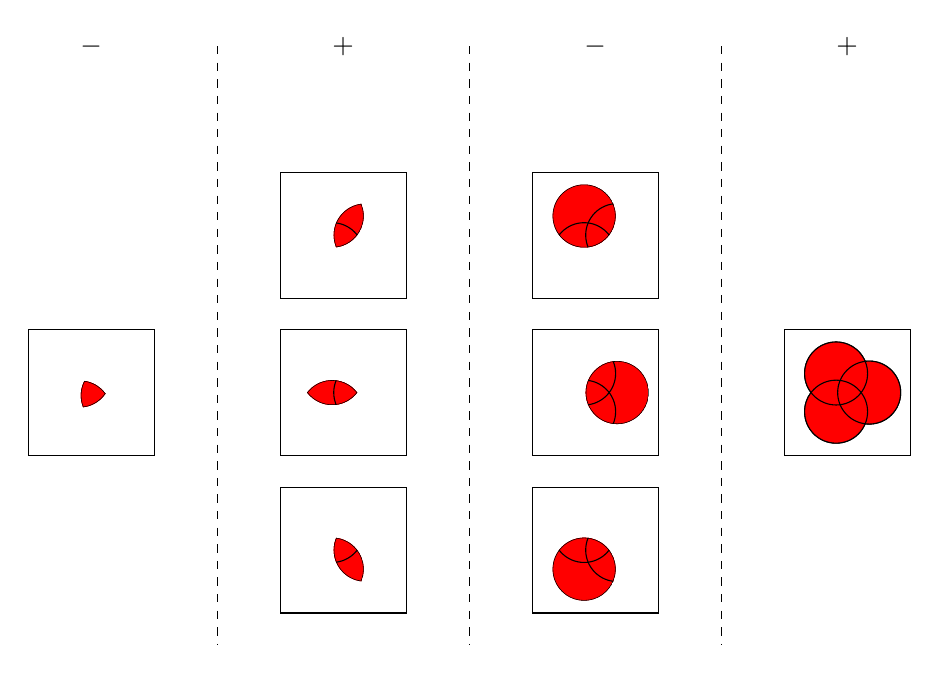
\begin{tikzpicture}[scale=.4]
\begin{scope}[shift={(-24,2)}]
\draw  (13,-3) rectangle (17,-7);
\clip (-17:15.2947) circle[radius=1];
\clip (-18:16.477) circle[radius=1];
\clip (-21:15.6861) circle[radius=1];
\fill[red] (-17:15.2947) circle[radius=1];
\fill[red] (-18:16.477) circle[radius=1];
\fill[red] (-21:15.6861) circle[radius=1];
\draw (-17:15.2947) circle[radius=1];
\draw (-18:16.477) circle[radius=1];
\draw (-21:15.6861) circle[radius=1];
\end{scope}\begin{scope}[shift={(15,-3)}]
\draw  (-2,2) rectangle (2,-2);
\draw (120:0.7) circle[radius=1];
\draw (0:0.7) circle[radius=1];
\draw (240:0.7) circle[radius=1];
\fill[red] (120:0.7) circle[radius=1];
\fill[red] (0:0.7) circle[radius=1];
\fill[red] (240:0.7) circle[radius=1];
\draw (120:0.7) circle[radius=1];
\draw (0:0.7) circle[radius=1];
\draw (240:0.7) circle[radius=1];
\end{scope}\begin{scope}[shift={(7,2)}]
\draw  (-2,2) rectangle (2,-2);
\clip (120:0.7) circle[radius=1];
\draw (0:0.7) circle[radius=1];
\draw (240:0.7) circle[radius=1];
\fill[red] (120:0.7) circle[radius=1];
\fill[red] (0:0.7) circle[radius=1];
\fill[red] (240:0.7) circle[radius=1];
\draw (120:0.7) circle[radius=1];
\draw (0:0.7) circle[radius=1];
\draw (240:0.7) circle[radius=1];
\end{scope}\begin{scope}[shift={(7,-3)}]
\draw  (-2,2) rectangle (2,-2);
\clip (0:0.7) circle[radius=1];
\draw (120:0.7) circle[radius=1];
\draw (240:0.7) circle[radius=1];
\fill[red] (120:0.7) circle[radius=1];
\fill[red] (0:0.7) circle[radius=1];
\fill[red] (240:0.7) circle[radius=1];
\draw (120:0.7) circle[radius=1];
\draw (0:0.7) circle[radius=1];
\draw (240:0.7) circle[radius=1];
\end{scope}\begin{scope}[shift={(7,-8)}]
\draw  (-2,2) rectangle (2,-2);
\clip (240:0.7) circle[radius=1];
\draw (120:0.7) circle[radius=1];
\draw (0:0.7) circle[radius=1];
\fill[red] (120:0.7) circle[radius=1];
\fill[red] (0:0.7) circle[radius=1];
\fill[red] (240:0.7) circle[radius=1];
\draw (120:0.7) circle[radius=1];
\draw (0:0.7) circle[radius=1];
\draw (240:0.7) circle[radius=1];
\end{scope}\begin{scope}[shift={(-1,2)}]
\draw  (-2,2) rectangle (2,-2);
\clip (120:0.7) circle[radius=1];
\clip (0:0.7) circle[radius=1];
\draw (240:0.7) circle[radius=1];
\fill[red] (120:0.7) circle[radius=1];
\fill[red] (0:0.7) circle[radius=1];
\fill[red] (240:0.7) circle[radius=1];
\draw (120:0.7) circle[radius=1];
\draw (0:0.7) circle[radius=1];
\draw (240:0.7) circle[radius=1];
\end{scope}\begin{scope}[shift={(-1,-3)}]
\draw  (-2,2) rectangle (2,-2);
\clip (120:0.7) circle[radius=1];
\clip (240:0.7) circle[radius=1];
\draw (0:0.7) circle[radius=1];
\fill[red] (120:0.7) circle[radius=1];
\fill[red] (0:0.7) circle[radius=1];
\fill[red] (240:0.7) circle[radius=1];
\draw (120:0.7) circle[radius=1];
\draw (0:0.7) circle[radius=1];
\draw (240:0.7) circle[radius=1];
\end{scope}\begin{scope}[shift={(-1,-8)}]
\draw  (-2,2) rectangle (2,-2);
\clip (0:0.7) circle[radius=1];
\clip (240:0.7) circle[radius=1];
\draw (120:0.7) circle[radius=1];
\fill[red] (120:0.7) circle[radius=1];
\fill[red] (0:0.7) circle[radius=1];
\fill[red] (240:0.7) circle[radius=1];
\draw (120:0.7) circle[radius=1];
\draw (0:0.7) circle[radius=1];
\draw (240:0.7) circle[radius=1];
\end{scope}
\node at (-9,8) {$-$};
\node at (-1,8) {$+$};
\node at (7,8) {$-$};
\node at (15,8) {$+$};
\draw[dashed] (-5,8) -- (-5,-11);
\draw[dashed] (3,8) -- (3,-11);
\draw[dashed] (11,8) -- (11,-11);
\end{tikzpicture}
\caption{Inclusion Exclusion says that the sum of the elements weighted with the signs listed is zero. }
\label{fig:incex}
\end{figure}
We will prove this theorem by using the tools of homological algebra.
\begin{notation}
If $U$ is a set, denote by $\Z_2\langle U \rangle$ the vector space which has $U$ as a basis. If $f: U\to V$ is a map of sets, we will similarly denote by $f: \Z_2\langle U \rangle \to \Z_2\langle V\rangle$ the induced map set by mapping the basis elements according to $f$. 
\end{notation} 
A covering $\mathcal U=\{U_i\}$ of $X$  is a collection of subsets $U_i\subset X$ so that  \[X=\bigcup_{i\in I} U_i.\]
To each covering of $X$ we will create an \emph{resolution complex} $CR_\bullet(\mathcal U)$.
\begin{definition}
Let $\mathcal U=\{U_i\}_{i\in I}$ be a covering of $X$. For each $J$ subset $i$, define the subset $U_J:=\cap_{i\in J} U_i$\footnote{Should $J=\emptyset,$ let $U_{\emptyset}=X$}, and as shorthand the associated vector space 
\[A_J:= \Z_2 \langle U_J\rangle. \]
Suppose that $J$ and $K$ differ by a single index. We will then write $J\lessdot K$. Notice that whenever $K\gtrdot J$ we have an inclusion map $i_{K\gtrdot J}:U_K\to U_J$, and therefore we get an associated map 
\[i_{K\gtrdot J}: A_K\to A_J.\]
We define the chain groups 
\[CR_k:=\bigoplus_{K\subset I, |K|=k} A_K\]
and define the differential map to be
\[\partial_k^{CR}:=\bigoplus_{K\gtrdot J} i_{K\gtrdot J}.\]
\end{definition}
Before we show that this gives us a chain complex, let's look at an example, and make an important note.

\begin{example}[Inclusion-Exclusion Complex]
\label{exam:inclusionexclusioncomplex}
Let suppose we have that  $X=U_1\cup U_2\cup U_3$, as in  \ref{fig:incex} . We can represent this data with the following diagram of resolutions:
\[	\begin{tikzcd}[row sep=small]
			\;&A_1  \cap A_2\arrow{r} \arrow{ddr} & A_1 \arrow{ddr}\\
			&\oplus&\oplus\\
			A_1\arrow{r} \arrow{uur} \arrow{ddr} \cap A_2\cap A_3 & A_1\cap A_3 \arrow{uur} \arrow{ddr}& A_2 \arrow{r} & A_1\cup A_2\cup A_3\\ 
			&\oplus&\oplus\\
			&A_2\cap A_3 \arrow{uur} \arrow{r} & A_3 \arrow{uur}
		\end{tikzcd}\]
Notice that each vertex of this cube represents a subset $K\subset\{1,2,3\}$. Each arrow in this diagram is represented by a pair $J\lessdot K$ where $J$ and $K$ differ by a single element. For each such pair $J,K$ denote by $i_{JK}$ the corresponding inclusion of subsets.\\
\end{example}
How does this chain complex help us prove the statement of inclusion exclusion? Notice that the Euler characteristic of this chain complex is 
\[
\sum_{k} \dim CR_k(\mathcal U)=|X|-\sum_{J\subset I}(-1)^{|J|} \left|\cap_{i\in J} U_i\right|. 
\]
If we can show that Euler Characteristic vanishes, we will have proven inclusion-exclusion.  
To show that this is a chain complex, we use the language of cones. 
\begin{lemma}
Let $\hat U_1$ be the elements of $X$ which only belong to $U_1$, and let $\hat A_1$ be it's associated vector space.  Let $\mathcal U_X=\{U_i\}_{i\in I}$ be a cover of $X$. Let $\mathcal U_{\cap}=\{U_i\cap U_1\}_{1\neq i\in I} $ be a cover for $U_1\setminus \hat A_1$. Let $\mathcal U_{\setminus}=\{U_i\}_{1\neq i\in I}$ be a cover for $X \setminus \hat U_1$. Suppose that $CR_\bullet(\mathcal U_\cup)$ and $CR_\bullet(\mathcal U_\cap)$ are chain complexes. Then there is a natural map 
\[i: CR_\bullet(\mathcal U_\cap)\to CR_\bullet(\mathcal U_\cup)\]
and $CR_\bullet(\mathcal U_X)=\cone(i)\oplus (\hat A_1\to \hat A_1)$
\end{lemma}
As always, a diagram explains the core concept of this proof:
\[\begin{tikzpicture}[commutative diagrams/every diagram]
\fill[red!10] (0,3) -- (-2.5,-0.5) -- (1.5,-0.5) -- (4,3) -- cycle;
\fill[blue!10] (-1.5,5.5) -- (-4,2) -- (0,2) -- (2.5,5.5) -- cycle;
\matrix[matrix of math nodes, name=m, commutative diagrams/every cell, row sep= 20, column sep = 30] {
\; & A_{12} & A_1 \\
			&\oplus&\oplus\\
A_{123}& A_{13}& A_2 & X\\
			&\oplus&\oplus\\
& A_{23} & A_3 \\};
\path[commutative diagrams/.cd, every arrow, every label]
(m-3-1) edge(m-1-2) edge (m-3-2) edge (m-5-2)
(m-1-2) edge(m-1-3) edge (m-3-3) 
(m-3-2) edge(m-1-3) edge (m-5-3) 
(m-5-2) edge(m-3-3) edge (m-5-3) 
(m-5-3) edge(m-3-4) 
(m-3-3) edge(m-3-4) 
(m-1-3) edge(m-3-4) 
;
\node at (1.5,7) {$CR_\bullet(\mathcal U_\cap \oplus A_1)$};
\node at (5,4) {$CR_\bullet(\mathcal U_\cup\oplus A_1)$};
\draw[->] (3,7) -- (4.5,4.5);
\end{tikzpicture}\]
The proof is a check of the definitions used to construct the chain complexes. More importantly, we get the following corollaries:
\begin{corollary}
The complexes $(CR_\bullet(\mathcal U)$ are in fact chain complexes.
\end{corollary}
\begin{proof}
One proves this by recursively defining $CR_\bullet(\mathcal U)=\cone(CR_\bullet(\mathcal U_\cap)\to CR_\bullet(\mathcal U_\cup)$ and inducting on the size of the cover $\mathcal U$.  If $\mathcal U=\{X\}$, then the associated chain complex is 
\[0 \to X\to X \to 0\]. 
\end{proof}
\begin{corollary}
The homology of the resolution complexes are trivial: $H_\bullet(CR_\bullet(\mathcal U))=0$, i.e. $CR_\bullet(\mathcal U)$ is exact. 
\end{corollary}
\begin{proof}
We again prove by induction on the size of the cover. As a base case, we can let  $\mathcal U=\{X\}$, then $H_\bullet(\mathcal U)=0$ trivially. \\
Now assume that we know by induction that $CR_\bullet(\mathcal U_\cap)$ and $ CR_\bullet(\mathcal U_\cup)$ have trivial homology. Since the cone of exact chain complexes is exact, we get $CR_\bullet(\mathcal U)$ is exact. 
\end{proof}
This allows us to prove the principle of inclusion-exclusion. 
\begin{corollary} Let $\mathcal U=\{U_i\}$ be a covering of $X$. Then
\[
0=|X|-\sum_{J\subset I}(-1)^{|J|} \left|\cap_{i\in J} U_i\right|. 
\]
\end{corollary}
\begin{proof}
Since $CR_\bullet(\mathcal U)$ is exact, 
\[0=\chi(CR_\bullet(\mathcal U))=|X|-\sum_{J\subset I}(-1)^{|J|} \left|\cap_{i\in J} U_i\right|.\]
\end{proof}
\section{Inclusion-Exclusion principles: The Zig-Zag Lemma} 
\label{append:inexzigzag}
Let's now use Inclusion-Exclusion to build up some more intuition on what homological algebra can get us. We will now work a little abstractly.
Let $\mathcal C$ be a collection of objects. Let's suppose that objects in this collection admit decompositions, so that we may write 
\[X=A\cup B\]
and for every such decomposition, we may also associate an objects called $A\cap B$. \\
A \emph{property} is a function $P: \mathcal C\to \N$ which assigns to each object a number. 
\begin{example}
Let our group of objects be $\Set$, the set of all finite sets. Then given $f: A\to X$, and $g: B\to X$, we have that $X=A\cup B$ if the map $f\sqcup g: A\sqcup B \to X$ was surjective. \\
In this case, we can also define $A\cap B$. The property that we're interested in the case of sets is their size, which defines a function $|\;\cdot \;|: \Set \to \N.$
\end{example}
\begin{example}
Let our group of objects be graphs. Similarly we have an idea of covering $G=H_1\cup H_2$, and an idea of intersection.\\
There are several different properties we could look at. We could look at $|V(G)|$, which measures the number of vertices, or $|E(G)|$, which measures the number of edges. \\
A more interesting property is the number of connected components, $b_0(G)$, or $b_1(G)$, the dimension of the cycle space.\\
A very difficult property to compute is $\gamma_G(k)$, which computes the number of $k$-colorings. 
\end{example}
Our goal is to come up with a general framework to understand how to compute properties with the framework of decompositions. 
\begin{definition}
A category $\mathcal C$ and a property $P$ satisfy an \emph{inclusion-exclusion principle} if for every decomposition $X=A\cup B$, we have 
\[P(X)=P(A)+P(B)-P(A\cap B).\]
\end{definition}
Sets, and sizes of sets is a classic example of a category and a property that obey the inclusion-exclusion principle. However, many properties do not satisfy the inclusion-exclusion principle. 
\begin{example}
Let $C_n$ be a cycle, and $C_n=P_{m_1}\cup P_{m_2}$ be a decomposition so that $P_{m_1}\cap P_{m_2}=\{u,v\}. $ Then we have that $b_0(C_n)=1$, but 
\[b_0(P_{m_1})+b_0(P_{m_2})-b_0(P_{m_1}\cap P_{m_2})=0.\]
This property does not have the inclusion-exclusion property
\end{example}
Though the inclusion-exclusion property does not hold, it almost holds, and the more subtle properties of graphs is what prevents the inclusion-exclusion properties from holding. However, we can access some of these properties by using homological algebra. 
\begin{definition}
Let $\mathcal C$ be a category, and $P: \mathcal C\to \N$ be a property. We say that $P$ obeys the \emph{homological inclusion-exclusion principle} if for all $X$, there exists a chain complex $P_\bullet(X)$ satisfying the following conditions:
\begin{itemize}
\item \emph{Recovery of $P$:} We have that $\dim H_0(P_\bullet(X))=P(X).$
\item \emph{Inclusion-Exclusion:} Whenever $X=A\cup B$, we have a short exact sequence:
\[0\to P_\bullet(A\cap B)\to P_\bullet(A)\oplus P_\bullet(B)\to P_\bullet(X)\to 0.\]
\end{itemize}
\end{definition}
Notice that satisfying a homological inclusion-exclusion principle is in a lot of ways like satisfying a inclusion-exclusion principle, in that 
\[\dim(P_0(X))= dim (P_0(A))+\dim(P_0(B))-\dim(P_0(A\cap B)).\]
While we don't get an actual inclusion exclusion principle from a homological inclusion-exclusion principle, we get something very close to the principle holding. In order to see the relation between inclusion-exclusion and homological inclusion-exclusion, we need a powerful lemma from homological algebra. 
\begin{theorem}[Zig-Zag Lemma]
Let $ A_\bullet,\partial^A_\bullet$ , $ B_\bullet,d^B_\bullet$ and $C_\bullet,d^C_\bullet$ be chain complexes. Given 
\[\begin{tikzcd} 0\arrow{r}&  A_\bullet \arrow{r}{f}& B_\bullet \arrow{r}{g} &C_\bullet \arrow{r} &0\end{tikzcd}\] a short exact sequence, there exists a unique map $\delta$ such that the following is a long exact sequence on homology:
\[\begin{tikzcd}[column sep=small] \cdots \arrow{r}{g_*}&H_{n+1}(C)\arrow{r}{\delta}& H_n ( A)\arrow{r}{f_*}& H_n( B)\arrow{r}{g_*}& H_n(C)\arrow{r}{\delta}& H_{n-1}( A)\arrow{r}{f_*}&\cdots \end{tikzcd}\] \label{lemma:zigzag}
\end{theorem}
Before we get into a proof of this theorem, let's quickly make a remark on the map $\delta$. On the one hand, the map is remarkable, as there is no reason to expect a map connecting $C\to A$. However, we've seen the existence of a long exact sequence that arises from a short exact sequence before when we looked at cones. \\
\begin{projectdescription}{Foo}
In a certain sense, this theorem says that \emph{all short exact sequences of chain complexes essentially arise from the cone sequence.} While we will not be able to prove this result in this class, one can make a version of this statement true by exploring the derived category and triangulated structures.  \label{proj:derived}
\end{projectdescription}
\begin{proof}
First, let's expand the original diagram:
\[\begin{tikzcd}
\; & \vdots   \arrow{d}{\partial} & \vdots\arrow{d}{\partial^B} &\vdots \arrow{d}{\partial^C}&\\
0\arrow{r}& A_{n+1}\arrow{d}{\partial_{n+1}}\arrow{r}{f_{n+1}} & B_{n+1}\arrow{d}{\partial^B_{n+1}}\arrow{r}{g_{n+1}} & C_{n+1}\arrow{d}{\partial^C_{n+1}}\arrow{r}&0\\
0\arrow{r}& A_{n  }\arrow{d}{\partial^A_{n  }}\arrow{r}{f_{n  }} & B_{n  }\arrow{d}{\partial^B_{n  }}\arrow{r}{g_{n  }} & C_{n  }\arrow{d}{\partial^C_{n  }}\arrow{r}&0\\
0\arrow{r}& A_{n-1}\arrow{d}{\partial^A_{n-1}}\arrow{r}{f_{n-1}} & B_{n-1}\arrow{d}{\partial^B_{n-1}}\arrow{r}{g_{n-1}} & C_{n-1}\arrow{d}{\partial^C_{n-1}}\arrow{r}&0\\
\;&\vdots&\vdots&\vdots&
\end{tikzcd}\]
We want to construct a function $\delta$ from $H_{n}(C)$ to $H_{n-1}(A)$. The following argument is an \emph{element chasing argument}, which can be a bit difficult to follow through; it's suggested that the reader write out the argument step-by-step at some point on their own to see where the maps come from.\\
Since this lemma contains several statements, we will check some of them and leave the remainder as exercises. 
\begin{claim}
There exists a canonical map $\delta: H_k(C)\to H_{k-1}(A).$
\end{claim}
As mentioned before, we should somewhat expect the existence of this map from our studies of cones. First, let's try and show that to a homology class $[\gamma]\in H_k(C)$, we can find an element in $A_{k-1}$  
\begin{itemize}
\item As the map $g_n$ is surjective, we know that we can pick an element in the preimage $\beta$ so that $g_n(\beta)=\gamma$. \emph{Notice that this is not a canonical choice!}
\[ 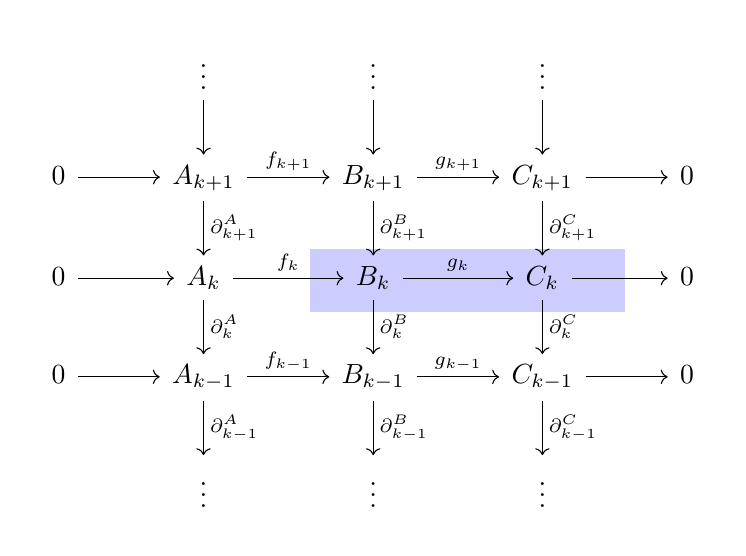
\begin{tikzpicture}
\usetikzlibrary{cd}


\fill[fill=blue!20]  (-0.8,3.2) rectangle (3.2,2.4);

\matrix[matrix of math nodes, name=m, commutative diagrams/every cell, row sep= 20, column sep = 30] {
\; & \vdots   & \vdots&\vdots &\\
0& A_{k+1} & B_{k+1} & C_{k+1}&0\\
0& A_{k} & B_{k} & C_{k}&0\\
0& A_{k-1} & B_{k-1} & C_{k-1}&0\\
\;&\vdots &\vdots &\vdots &\\};
\path[commutative diagrams/.cd, every arrow, every label]
(m-1-2) edge (m-2-2)    (m-1-3) edge (m-2-3)     (m-1-4) edge (m-2-4)
(m-2-1) edge (m-2-2)
(m-2-2) edge node {$\partial^A_{k+1}$} (m-3-2)    edge node {$f_{k+1}$} (m-2-3)      
(m-2-3)edge node {$\partial^B_{k+1}$} (m-3-3)    edge node {$g_{k+1}$}  (m-2-4)  
(m-2-4) edge node {$\partial^C_{k+1}$}(m-3-4)  edge (m-2-5)  

(m-3-1) edge (m-3-2)
(m-3-2) edge node {$\partial^A_{k}$} (m-4-2)    edge node {$f_{k}$} (m-3-3)      
(m-3-3)edge node {$\partial^B_{k}$} (m-4-3)    edge node {$g_{k}$}  (m-3-4)  
(m-3-4) edge node {$\partial^C_{k}$}(m-4-4)  edge (m-3-5)  

(m-4-1) edge (m-4-2)
(m-4-2) edge node {$\partial^A_{k-1}$} (m-5-2)    edge node {$f_{k-1}$} (m-4-3)      
(m-4-3)edge node {$\partial^B_{k-1}$} (m-5-3)    edge node {$g_{k-1}$}  (m-4-4)  
(m-4-4) edge node {$\partial^C_{k-1}$}(m-5-4)  edge (m-4-5)  
;
\end{tikzpicture}\]
\item We can apply $\partial^B_n(\beta)$ and we wind up with an element in $B_{n-1}$. Using that $g_{n-1}$ is a chain map, we get that  
\[g_{n-1} \partial^B_n(\beta)= \partial^Cg_n(\beta)=\partial^C \gamma =0\]
where the second equality comes from the fact that $\gamma$ represents a homology class. 
\[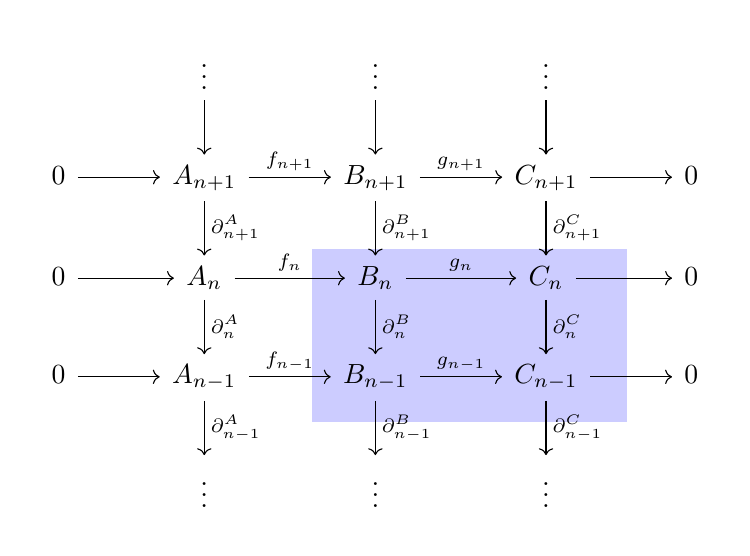
\begin{tikzpicture}
\usetikzlibrary{cd}

\fill[fill=blue!20]  (-0.8,3.2) rectangle (3.2,1);
\matrix[matrix of math nodes, name=m, commutative diagrams/every cell, row sep= 20, column sep = 30] {
\; & \vdots   & \vdots&\vdots &\\
0& A_{n+1} & B_{n+1} & C_{n+1}&0\\
0& A_{n} & B_{n} & C_{n}&0\\
0& A_{n-1} & B_{n-1} & C_{n-1}&0\\
\;&\vdots &\vdots &\vdots &\\};
\path[commutative diagrams/.cd, every arrow, every label]
(m-1-2) edge (m-2-2)    (m-1-3) edge (m-2-3)     (m-1-4) edge (m-2-4)
(m-2-1) edge (m-2-2)
(m-2-2) edge node {$\partial^A_{n+1}$} (m-3-2)    edge node {$f_{n+1}$} (m-2-3)      
(m-2-3)edge node {$\partial^B_{n+1}$} (m-3-3)    edge node {$g_{n+1}$}  (m-2-4)  
(m-2-4) edge node {$\partial^C_{n+1}$}(m-3-4)  edge (m-2-5)  

(m-3-1) edge (m-3-2)
(m-3-2) edge node {$\partial^A_{n}$} (m-4-2)    edge node {$f_{n}$} (m-3-3)      
(m-3-3)edge node {$\partial^B_{n}$} (m-4-3)    edge node {$g_{n}$}  (m-3-4)  
(m-3-4) edge node {$\partial^C_{n}$}(m-4-4)  edge (m-3-5)  

(m-4-1) edge (m-4-2)
(m-4-2) edge node {$\partial^A_{n-1}$} (m-5-2)    edge node {$f_{n-1}$} (m-4-3)      
(m-4-3)edge node {$\partial^B_{n-1}$} (m-5-3)    edge node {$g_{n-1}$}  (m-4-4)  
(m-4-4) edge node {$\partial^C_{n-1}$}(m-5-4)  edge (m-4-5)  
;
\end{tikzpicture}\]
\item Since $\partial^B_n(\beta)\in \ker g_{n-}1$, and the sequence is chain complexes is exact, we know that $\partial^B_(\beta)\in \im f_{n-1}$. Since $f_{n-1}$ is injective, we know that there is unique $\alpha$ corresponding to this $\beta$ so that $f_{n-1}(\alpha)=\partial^B(\beta).$
\[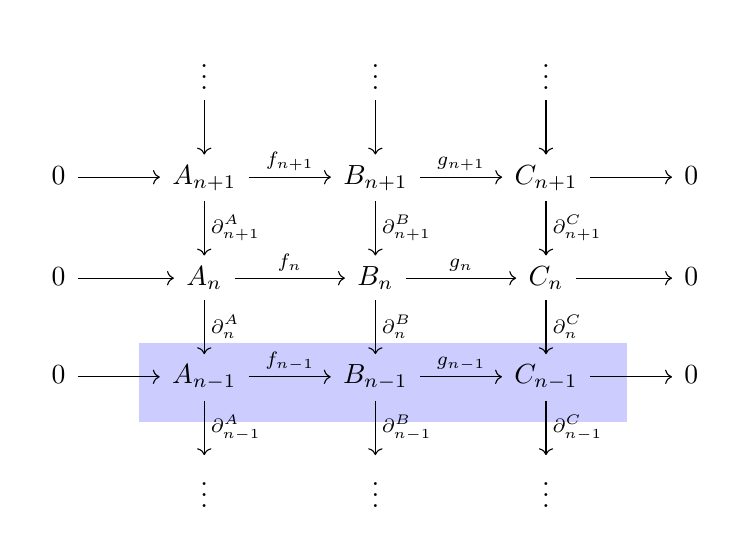
\begin{tikzpicture}
\usetikzlibrary{cd}


\fill[fill=blue!20]  (-3,2) rectangle (3.2,1);

\matrix[matrix of math nodes, name=m, commutative diagrams/every cell, row sep= 20, column sep = 30] {
\; & \vdots   & \vdots&\vdots &\\
0& A_{n+1} & B_{n+1} & C_{n+1}&0\\
0& A_{n} & B_{n} & C_{n}&0\\
0& A_{n-1} & B_{n-1} & C_{n-1}&0\\
\;&\vdots &\vdots &\vdots &\\};
\path[commutative diagrams/.cd, every arrow, every label]
(m-1-2) edge (m-2-2)    (m-1-3) edge (m-2-3)     (m-1-4) edge (m-2-4)
(m-2-1) edge (m-2-2)
(m-2-2) edge node {$\partial^A_{n+1}$} (m-3-2)    edge node {$f_{n+1}$} (m-2-3)      
(m-2-3)edge node {$\partial^B_{n+1}$} (m-3-3)    edge node {$g_{n+1}$}  (m-2-4)  
(m-2-4) edge node {$\partial^C_{n+1}$}(m-3-4)  edge (m-2-5)  

(m-3-1) edge (m-3-2)
(m-3-2) edge node {$\partial^A_{n}$} (m-4-2)    edge node {$f_{n}$} (m-3-3)      
(m-3-3)edge node {$\partial^B_{n}$} (m-4-3)    edge node {$g_{n}$}  (m-3-4)  
(m-3-4) edge node {$\partial^C_{n}$}(m-4-4)  edge (m-3-5)  

(m-4-1) edge (m-4-2)
(m-4-2) edge node {$\partial^A_{n-1}$} (m-5-2)    edge node {$f_{n-1}$} (m-4-3)      
(m-4-3)edge node {$\partial^B_{n-1}$} (m-5-3)    edge node {$g_{n-1}$}  (m-4-4)  
(m-4-4) edge node {$\partial^C_{n-1}$}(m-5-4)  edge (m-4-5)  
;
\end{tikzpicture}\]
\item We initially define $\delta[\gamma]=\alpha$. 
\end{itemize}
We now need to show that $\alpha$ is a homology class, that is, that $\partial_{k-1}^A(\alpha)=0$. 
\begin{itemize}
\item Look at $\partial_{k-1}^A(\alpha)$. Since this diagram is commutative, we have that $f_{k-2} \partial^A_{k-1}(\alpha)= \partial^B_{k-1}f_{k-1}(\alpha).$
\[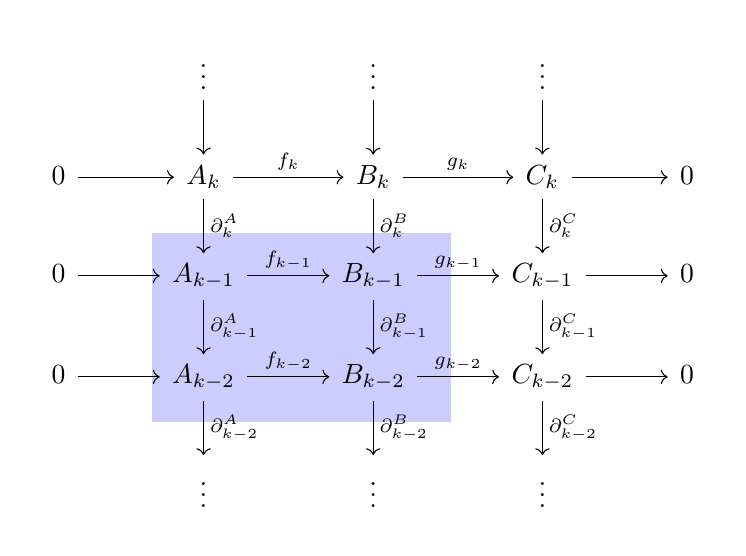
\begin{tikzpicture}
\usetikzlibrary{cd}


\fill[fill=blue!20]  (-2.8,3.4) rectangle (1,1);

\matrix[matrix of math nodes, name=m, commutative diagrams/every cell, row sep= 20, column sep = 30] {
\; & \vdots   & \vdots&\vdots &\\
0& A_{k} & B_{k} & C_{k}&0\\
0& A_{k-1} & B_{k-1} & C_{k-1}&0\\
0& A_{k-2} & B_{k-2} & C_{k-2}&0\\
\;&\vdots &\vdots &\vdots &\\};
\path[commutative diagrams/.cd, every arrow, every label]
(m-1-2) edge (m-2-2)    (m-1-3) edge (m-2-3)     (m-1-4) edge (m-2-4)
(m-2-1) edge (m-2-2)
(m-2-2) edge node {$\partial^A_{k}$} (m-3-2)    edge node {$f_{k}$} (m-2-3)      
(m-2-3)edge node {$\partial^B_{k}$} (m-3-3)    edge node {$g_{k}$}  (m-2-4)  
(m-2-4) edge node {$\partial^C_{k}$}(m-3-4)  edge (m-2-5)  

(m-3-1) edge (m-3-2)
(m-3-2) edge node {$\partial^A_{k-1}$} (m-4-2)    edge node {$f_{k-1}$} (m-3-3)      
(m-3-3)edge node {$\partial^B_{k-1}$} (m-4-3)    edge node {$g_{k-1}$}  (m-3-4)  
(m-3-4) edge node {$\partial^C_{k-1}$}(m-4-4)  edge (m-3-5)  

(m-4-1) edge (m-4-2)
(m-4-2) edge node {$\partial^A_{k-2}$} (m-5-2)    edge node {$f_{k-2}$} (m-4-3)      
(m-4-3)edge node {$\partial^B_{k-2}$} (m-5-3)    edge node {$g_{k-2}$}  (m-4-4)  
(m-4-4) edge node {$\partial^C_{k-2}$}(m-5-4)  edge (m-4-5)  
;
\end{tikzpicture}\]
\item Recalling or definition of $\alpha$, we know that $f_{k-1}(\alpha)= \partial^B_{k}(\beta)$, so $\partial_{k-1}^B(\partial^B_k(\beta)= f_{k-2}(\partial_{k-1}\alpha)=0$. Since $f_{k-2}$ is injective, we get that $\partial_{k-1}\alpha)=0$. 
\[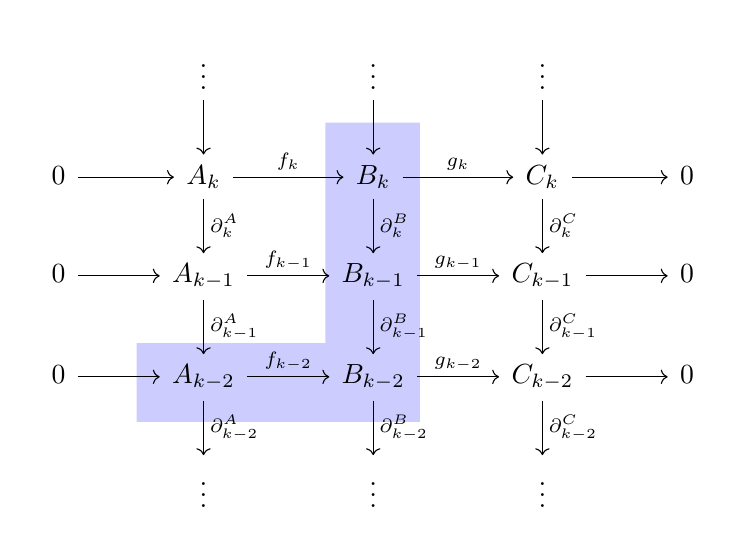
\begin{tikzpicture}
\usetikzlibrary{cd}


\fill[blue!20] (-3,2) -- (-3,1) -- (0.6,1) -- (0.6,4.8) -- (-0.6,4.8) -- (-0.6,2) -- cycle;

\matrix[matrix of math nodes, name=m, commutative diagrams/every cell, row sep= 20, column sep = 30] {
\; & \vdots   & \vdots&\vdots &\\
0& A_{k} & B_{k} & C_{k}&0\\
0& A_{k-1} & B_{k-1} & C_{k-1}&0\\
0& A_{k-2} & B_{k-2} & C_{k-2}&0\\
\;&\vdots &\vdots &\vdots &\\};
\path[commutative diagrams/.cd, every arrow, every label]
(m-1-2) edge (m-2-2)    (m-1-3) edge (m-2-3)     (m-1-4) edge (m-2-4)
(m-2-1) edge (m-2-2)
(m-2-2) edge node {$\partial^A_{k}$} (m-3-2)    edge node {$f_{k}$} (m-2-3)      
(m-2-3)edge node {$\partial^B_{k}$} (m-3-3)    edge node {$g_{k}$}  (m-2-4)  
(m-2-4) edge node {$\partial^C_{k}$}(m-3-4)  edge (m-2-5)  

(m-3-1) edge (m-3-2)
(m-3-2) edge node {$\partial^A_{k-1}$} (m-4-2)    edge node {$f_{k-1}$} (m-3-3)      
(m-3-3)edge node {$\partial^B_{k-1}$} (m-4-3)    edge node {$g_{k-1}$}  (m-3-4)  
(m-3-4) edge node {$\partial^C_{k-1}$}(m-4-4)  edge (m-3-5)  

(m-4-1) edge (m-4-2)
(m-4-2) edge node {$\partial^A_{k-2}$} (m-5-2)    edge node {$f_{k-2}$} (m-4-3)      
(m-4-3)edge node {$\partial^B_{k-2}$} (m-5-3)    edge node {$g_{k-2}$}  (m-4-4)  
(m-4-4) edge node {$\partial^C_{k-2}$}(m-5-4)  edge (m-4-5)  
;
\end{tikzpicture}\]
\end{itemize}
Finally, when we constructed the class $\alpha$, we had to make a choice of $\beta=g_k^{-1}(\gamma)$. Let's show that the homology class of $\alpha$ does not depend on the choice of $\beta$ lifting $\alpha$. 
\begin{itemize}
\item Suppose that $\beta, \beta'$ are two different liftings of $\gamma$ so that $g_k(\beta)-g_k(\beta')=0$. We want to show that the associated classes $[\alpha], [\alpha']$ are homologous. Since $g_k(\beta-\beta')=0$, there exists a class $f_k^{-1}(\beta-\beta')$ due to exactness of the row. 
 \[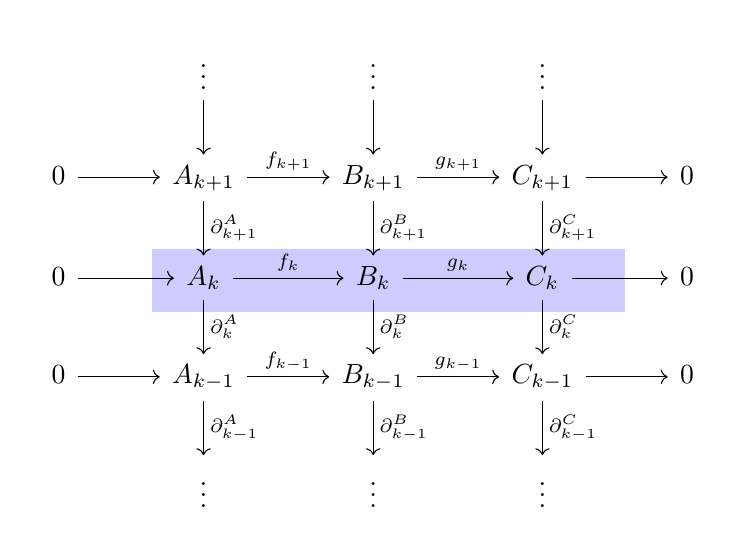
\begin{tikzpicture}
\usetikzlibrary{cd}
\fill[fill=blue!20]  (-2.8,3.2) rectangle (3.2,2.4);

\matrix[matrix of math nodes, name=m, commutative diagrams/every cell, row sep= 20, column sep = 30] {
\; & \vdots   & \vdots&\vdots &\\
0& A_{k+1} & B_{k+1} & C_{k+1}&0\\
0& A_{k} & B_{k} & C_{k}&0\\
0& A_{k-1} & B_{k-1} & C_{k-1}&0\\
\;&\vdots &\vdots &\vdots &\\};
\path[commutative diagrams/.cd, every arrow, every label]
(m-1-2) edge (m-2-2)    (m-1-3) edge (m-2-3)     (m-1-4) edge (m-2-4)
(m-2-1) edge (m-2-2)
(m-2-2) edge node {$\partial^A_{k+1}$} (m-3-2)    edge node {$f_{k+1}$} (m-2-3)      
(m-2-3)edge node {$\partial^B_{k+1}$} (m-3-3)    edge node {$g_{k+1}$}  (m-2-4)  
(m-2-4) edge node {$\partial^C_{k+1}$}(m-3-4)  edge (m-2-5)  

(m-3-1) edge (m-3-2)
(m-3-2) edge node {$\partial^A_{k}$} (m-4-2)    edge node {$f_{k}$} (m-3-3)      
(m-3-3)edge node {$\partial^B_{k}$} (m-4-3)    edge node {$g_{k}$}  (m-3-4)  
(m-3-4) edge node {$\partial^C_{k}$}(m-4-4)  edge (m-3-5)  

(m-4-1) edge (m-4-2)
(m-4-2) edge node {$\partial^A_{k-1}$} (m-5-2)    edge node {$f_{k-1}$} (m-4-3)      
(m-4-3)edge node {$\partial^B_{k-1}$} (m-5-3)    edge node {$g_{k-1}$}  (m-4-4)  
(m-4-4) edge node {$\partial^C_{k-1}$}(m-5-4)  edge (m-4-5)  
;
\end{tikzpicture}\]
\item Due to commutivity of the highlighted square, we have that $f_{k-1}\partial_k^A(f^{-1}_k(\beta-\beta')= \partial^B_k(\beta-\beta')=f_{k-1}(\alpha-\alpha')$. Due to the injectivity of $f_{k-1}$, we conclude that $\alpha-\alpha'= \partial_k^A(f^{-1}_k(\beta-\beta')$, so these two classes are cohomologous. 
\[ 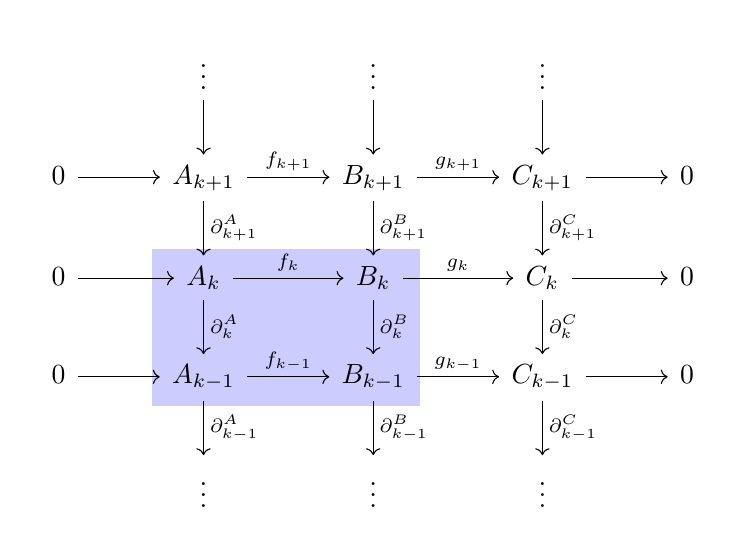
\begin{tikzpicture}
\usetikzlibrary{cd}


\fill[fill=blue!20]  (-2.8,3.2) rectangle (0.6,1.2);

\matrix[matrix of math nodes, name=m, commutative diagrams/every cell, row sep= 20, column sep = 30] {
\; & \vdots   & \vdots&\vdots &\\
0& A_{k+1} & B_{k+1} & C_{k+1}&0\\
0& A_{k} & B_{k} & C_{k}&0\\
0& A_{k-1} & B_{k-1} & C_{k-1}&0\\
\;&\vdots &\vdots &\vdots &\\};
\path[commutative diagrams/.cd, every arrow, every label]
(m-1-2) edge (m-2-2)    (m-1-3) edge (m-2-3)     (m-1-4) edge (m-2-4)
(m-2-1) edge (m-2-2)
(m-2-2) edge node {$\partial^A_{k+1}$} (m-3-2)    edge node {$f_{k+1}$} (m-2-3)      
(m-2-3)edge node {$\partial^B_{k+1}$} (m-3-3)    edge node {$g_{k+1}$}  (m-2-4)  
(m-2-4) edge node {$\partial^C_{k+1}$}(m-3-4)  edge (m-2-5)  

(m-3-1) edge (m-3-2)
(m-3-2) edge node {$\partial^A_{k}$} (m-4-2)    edge node {$f_{k}$} (m-3-3)      
(m-3-3)edge node {$\partial^B_{k}$} (m-4-3)    edge node {$g_{k}$}  (m-3-4)  
(m-3-4) edge node {$\partial^C_{k}$}(m-4-4)  edge (m-3-5)  

(m-4-1) edge (m-4-2)
(m-4-2) edge node {$\partial^A_{k-1}$} (m-5-2)    edge node {$f_{k-1}$} (m-4-3)      
(m-4-3)edge node {$\partial^B_{k-1}$} (m-5-3)    edge node {$g_{k-1}$}  (m-4-4)  
(m-4-4) edge node {$\partial^C_{k-1}$}(m-5-4)  edge (m-4-5)  
;
\end{tikzpicture}\]
\end{itemize}
This completes the proof that the map $\delta$ is well defined on homology. Now we will show some of the exactness statements. 
\begin{claim}
The sequence of homology groups 
\[H_k(B)\xrightarrow{g_k} H_k(C)\xrightarrow{\delta_k} H_{k-1}(A)\]
is exact. 
\end{claim}
In order to prove this claim, we need to show that $\ker(\delta)\subset \im(g_k)$, and $\im (g_k)\subset \ker \delta$. 
\begin{itemize}
\item To show that $\im(g_k)\subset \ker \delta$, it suffices to show that the composition $\delta_k \circ g_k=0$. Let $[\beta]\in H_k(B)$ be a homology class. Then $[\delta_k g_k(\beta)]= [f_{k-1}^{-1}(\partial^B_k\beta)]. $ Since $[\beta]$ is a class in homology, the boundary map starts by computing $\partial^B_k\beta=0$, and we conclude that $\delta_k (g_k(\beta))=0$. 
\item To show that the $\ker(\delta_k)\subset \im (g_k)$, let $\gamma$ be an element so that $\delta_k[\gamma]=0$. Since the map $g_k: B_k\to C_k$ is surjective, we might hope that $\beta=g^{-1}_k\gamma$, a choice of lift of $\gamma$, is a class in homology. So we need to show that $\partial^B_k(\beta)=0$. By commutivity of the lower right square, we have that 
$\partial^B_k(\beta)=f_{k-1}(\delta(\gamma))=0.$
\[ 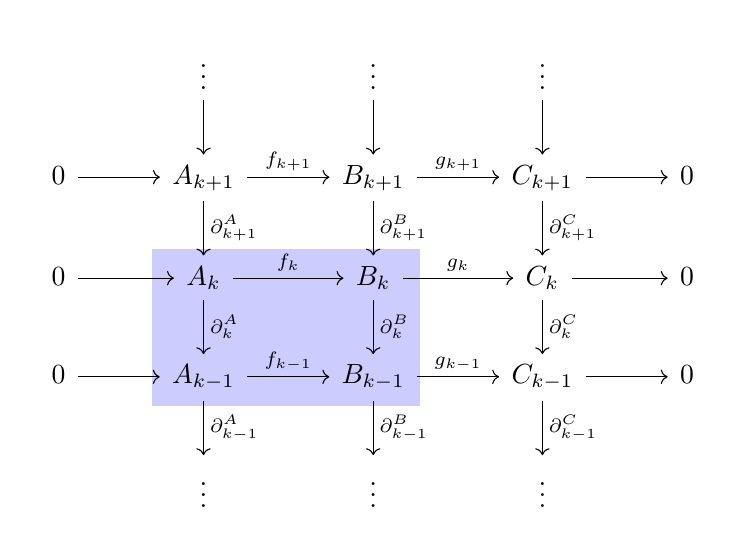
\begin{tikzpicture}
\usetikzlibrary{cd}


\fill[fill=blue!20]  (-2.8,3.2) rectangle (0.6,1.2);

\matrix[matrix of math nodes, name=m, commutative diagrams/every cell, row sep= 20, column sep = 30] {
\; & \vdots   & \vdots&\vdots &\\
0& A_{k+1} & B_{k+1} & C_{k+1}&0\\
0& A_{k} & B_{k} & C_{k}&0\\
0& A_{k-1} & B_{k-1} & C_{k-1}&0\\
\;&\vdots &\vdots &\vdots &\\};
\path[commutative diagrams/.cd, every arrow, every label]
(m-1-2) edge (m-2-2)    (m-1-3) edge (m-2-3)     (m-1-4) edge (m-2-4)
(m-2-1) edge (m-2-2)
(m-2-2) edge node {$\partial^A_{k+1}$} (m-3-2)    edge node {$f_{k+1}$} (m-2-3)      
(m-2-3)edge node {$\partial^B_{k+1}$} (m-3-3)    edge node {$g_{k+1}$}  (m-2-4)  
(m-2-4) edge node {$\partial^C_{k+1}$}(m-3-4)  edge (m-2-5)  

(m-3-1) edge (m-3-2)
(m-3-2) edge node {$\partial^A_{k}$} (m-4-2)    edge node {$f_{k}$} (m-3-3)      
(m-3-3)edge node {$\partial^B_{k}$} (m-4-3)    edge node {$g_{k}$}  (m-3-4)  
(m-3-4) edge node {$\partial^C_{k}$}(m-4-4)  edge (m-3-5)  

(m-4-1) edge (m-4-2)
(m-4-2) edge node {$\partial^A_{k-1}$} (m-5-2)    edge node {$f_{k-1}$} (m-4-3)      
(m-4-3)edge node {$\partial^B_{k-1}$} (m-5-3)    edge node {$g_{k-1}$}  (m-4-4)  
(m-4-4) edge node {$\partial^C_{k-1}$}(m-5-4)  edge (m-4-5)  
;
\end{tikzpicture}\]

\end{itemize}
\begin{claim}
The sequence of homology groups  
\[H_{k+1}(C)\xrightarrow{\delta_{k+1}} H_k(A)\xrightarrow{f_k} H_k(B)\]
is exact. 
\end{claim}
\end{proof}


\section{Chain Homotopy}
Homological algebra is ultimately the study of which chain complexes are isomorphic to eachother in a homological way.
\label{append:chainhomotopy}
\begin{definition} \label{def:quasiisomorphism} Let $f:A_\bullet \to B_\bullet$ be a chain map. Then we say that $f$ is a  \emph{quasi-isomorphism} if the induced map on homology, $f_*:H_i(\mathcal A)\to H_i(\mathcal B)$ are isomorphisms of homology groups. \end{definition}
Notice that while every isomorphism which is a chain map gives us a quasi-isomorphism, a chain map need not be an isomorphism to be a quasi-isomorphism. 
\begin{example}
Not isomorphic, but quasi-isomorphic. 
\end{example}
Similarly, even if $(A, \partial)$ and $(B, \partial)$ have isomorphic homology groups, they need to not be quasi-isomorphic. 
\begin{example}
It is not necessarily the case that if two chain complexes have isomorphic homology that those two complexes are quasi isomorphic. 
\end{example}
Even though $f_\bullet: A_\bullet\to B_\bullet$ is a quasi-isomorphism, there is no guarantee that there exists $g_\bullet: B_\bullet\to A_\bullet$ so that the maps $(g\circ f)_k: H_k(A)\to H_k(A)$ is the identity. In other words, there is no need for inverses to exists to quasi-isomorphism on either the chain or homological level. If such a map exists, we call it a \emph{quasi-inverse}. 
\begin{example}
Chain Complexes with no quasi-inverse.
\end{example}
It is usually hard come up with an interpretation of where a quasi-isomorphism comes from; in general the question if two maps $f,g :A_\bullet\to B_\bullet$ do the same thing on homology is hard to get some intuition on. As a proxy to showing that two maps have the same definition on homology, we introduce an idea from topology: that of a \emph{homotopy.}

\begin{definition} Let $(A,\partial^A)$ and $(B, \partial^B)$ be chain complexes. Let $f_\bullet:A_\bullet\to B_\bullet$ and $g_\bullet:A_\bullet \to B_\bullet$ be chain maps. Then we say that $f$ is \emph{chain homotopic} to $g$ if there exists a series of maps (called a \emph{chain homotopy}) $h_i:A_i\to B_{i+1}$ such that $$f-g=\partial^B h_{i}+h_{i-1}\partial^A$$ We write that $f\sim g$. \end{definition}

Here's a diagram that helps visualize the maps involved in a chain homotopy.
\[\begin{tikzcd}[column sep=2cm]
\cdots \arrow{r}{\partial^A} & A_{i+1}\arrow[bend left]{d}[description]{f} \arrow[bend right]{d}[description]{g}\arrow{dl}[description]{h_{i+1}} \arrow{r}{\partial^A} & A_{i}\arrow[bend left]{d}[description]{f} \arrow[bend right]{d}[description]{g}\arrow{dl}[description]{h_{i}} \arrow{r}{\partial^A}& A_{i-1} \arrow[bend left]{d}[description]{f} \arrow[bend right]{d}[description]{g}\arrow{dl}[description]{h_{i-1}}\arrow{r}{\partial^A}& \cdots \arrow{dl}[description]{h_{i-2}}\\
\cdots \arrow{r}{\partial^B} & B_{i+1} \arrow{r}{\partial^B} & B_{i} \arrow{r}{\partial^B}& B_{i-1} \arrow{r}{\partial^B}& \cdots \\
\end{tikzcd}\]
It can be difficult to get an intuition on what a chain homotopy between two map constitutes. One interpretation comes from topology; for every element $x$, the difference between $f(x)$ and $g(x)$ can be expressed as a cylinder connecting $f(x), g(x)$. This bears resemblance to the definition of a homotopy between two maps in point-set topology. \\
\begin{example} An example of a chain homotopy will go here!
\end{example}
One thing worth pointing out is that we don't have any condition of compatibility with the differential for the homotopy maps $h_k:A_k\to B_{k+1}$; they are allowed to be as crazy as need be. \\
Chain homotopy is especially useful for the following lemma:
\begin{lemma}
Suppose that $f_\bullet, g_\bullet: A_\bullet\to B_\bullet$ are chain homotopic chain maps. Then they are the same map on homology, in the sense that 
\[f_k[x]=g_k[x]\]
for every $[x]\in H_k(A). $
\end{lemma}
\begin{proof}
What we want to show is that $f_k-g_k= \partial^B_{k+1} h_{k}+h_{k-1}\partial^A_k$, then for every $[a]\in H_k(A)$, there exists $b\in C_{k+1}(B)$ with 
\[f_k(a)-g_k(a)=\partial_{k+1}(b).\]
The homotopy gives us a natural for $b$ is; we can let $b=h_k(a)$. Taking our definition of homotopy shows 
\begin{align*}f_k(a)-g_k(a)=&\partial^B_{k+1} h_{k}(a)+h_{k-1}\partial^A_k(a)\\
\intertext{ As $a$ represents a class in homology} 
=& \partial^B_{k+1} h_{k}(a)= \partial^B_{k+1}(b). \end{align*}
\end{proof}


This next claim shows the usefulness of chain homotopies:
\begin{lemma} Let $f:\mathcal A\to\mathcal B$ and $g:\mathcal B\to\mathcal A$ be chain maps. Suppose that $g\circ f\sim 1_{\mathcal A}$ and $g\circ f \sim 1_{\mathcal B}$. Then $f$ and $g$ are quasi-isomorphisms.
\begin{proof}
Let's start with a diagram.
$$\begin{tikzcd}[column sep=2cm]
\cdots \arrow[crossing over]{r}[near start]{d'} & A_{i+1} \arrow{r}{d}\arrow{ddl}[near start, description]{h} \arrow{d}[description]{f}\arrow[bend left]{dd}&  A_{i} \arrow{r}{d}\arrow{d}[description]{f}\arrow[bend left]{dd} \arrow{ddl}[near start, description]{h}& A_{i-1} \arrow{d}[description]{f}\arrow{r}{d}\arrow[bend left]{dd}\arrow{ddl}[near start, description]{h}& \cdots \\
\cdots \arrow[crossing over]{r}[near start]{d'} & B_{i+1} \arrow[crossing over]{r}[near start]{d'}\arrow{d}[description]{g}&  B_{i} \arrow[crossing over]{r}[near start]{d'}\arrow{d}[description]{g}& B_{i-1}\arrow{d}[description]{g}\arrow[crossing over]{r}[near start]{d'}& \cdots \\
\cdots \arrow[crossing over]{r}[near start]{d'} & A_{i+1} \arrow{r}{d}            &   A_{i} \arrow{r}{d}             & A_{i-1}\arrow{r}{d}             & \cdots \\
\end{tikzcd}$$
The homotopy to the identity map gives us that there exists $h$ such that $g\circ f- 1_{\mathcal A}=dh^{i}+h^{i-1}d$. Suppose that $v\in H_i{A}$. Then $v$ is in the kernel of $d$, so $h^{i-1}d(v)=h^{i-1}(0)=0$. We have that therefore $g\circ f - 1_{\mathcal A}\in \im(d)$, which is to say that on homology $g\circ f = 1_{\mathcal A}$, as we mod out by $\im(d)$ when we take homology.\\
Of course, a similar proof shows that $f\circ g=1_{\mathcal A}$
\end{proof}
\end{lemma}
\section{Snake Lemma}
\begin{comment}
Therefore, to show that a morphism is a quasi-isomorphism, one can just show that it is homotopic to the identity. As homotopies form an equivalence relationship on the set of morphisms, we can quotient out by homotopies to arrive a new category, the homotopy category of chain complexes$\C$. In this category, $f=g$ if $f\sim g$; in particular, maps who are isomorphisms in the homotopy category are quasi-isomorphisms in the original chain category. We call this category $\K(\C)$ .
Now, we will introduce the most powerful theorem for homology theory.
\begin{theorem}{Zig-Zag Lemma}
Let $\mathcal A,\partial_\bullet$ , $\mathcal B,d'_\bullet$ and $\C,d''_\bullet$ be chain complexes. Given $$\begin{tikzcd} 0\arrow{r}& \mathcal A\arrow{r}{f}&\mathcal B\arrow{r}{g} &\C\arrow{r}&0\end{tikzcd}$$ a short exact sequence, there exists a unique map $\delta$ such that the following is a long exact sequence on homology:
$$\begin{tikzcd}[column sep=small] \cdots \arrow{r}{g_*}&H_{n+1}(\C)\arrow{r}{\delta}& H_n (\mathcal A)\arrow{r}{f_*}& H_n(\mathcal B)\arrow{r}{g_*}& H_n(\C)\arrow{r}{\delta}& H_{n-1}(\mathcal A)\arrow{r}{f_*}&\cdots \end{tikzcd}$$
\begin{proof}
First, let's expand the original diagram:
\[\begin{tikzcd}
\; & \vdots   \arrow{d}{\partial} & \vdots\arrow{d}{\partial^B} &\vdots \arrow{d}{\partial ^C}&\\
0\arrow{r}& A_{n+1}\arrow{d}{\partial_{n+1}^A}\arrow{r}{f_{n+1}} & B_{n+1}\arrow{d}{\partial^B_{n+1}}\arrow{r}{g_{n+1}} & C_{n+1}\arrow{d}{\partial^C_{n+1}}\arrow{r}&0\\
0\arrow{r}& A_{n  }\arrow{d}{\partial^A_{n  }}\arrow{r}{f_{n  }} & B_{n  }\arrow{d}{d^B_{n  }}\arrow{r}{g_{n  }} & C_{n  }\arrow{d}{d^C_{n  }}\arrow{r}&0\\
0\arrow{r}& A_{n-1}\arrow{d}{\partial^A_{n-1}}\arrow{r}{f_{n-1}} & B_{n-1}\arrow{d}{d^B_{n-1}}\arrow{r}{g_{n-1}} & C_{n-1}\arrow{d}{d^C_{n-1}}\arrow{r}&0\\
\;&\vdots&\vdots&\vdots&
\end{tikzcd}\]
We want to construct a function $\delta$ from $H_{n}(\C)$ to $H_{n-1}(\mathcal A)$. Select a $[c]\in H_n(\C)$. Then lift it to $c\in C_n$. Take an element $b$ in the preimage of $c$ along $g_n$. Then as $d''_n(g_n(b))=d''_n(c)=0$, we have by commutivity of the diagram that $g_{n-1}(d'_n(b))=0$. Therefore, $\partial_n(b)\in \ker g_{n-1}$. However, $\ker g_{n-1}=\im f_{n-1}$ by exactness of the rows. There therefore exists unique $a\in A_{n-1}$ such that $f_{n-1}(a)=\partial_n(b)$. We choose the representive of  $a$ in $H_{n-1}(\mathcal A)$ to be $\delta(c)$. \\Now we have to show that this $a$ is independent of choice of $b$. Suppose instead we choose $b'$ in the preimage of $c$ along $g_n$. Let $d'_n(b')$ lift instead to $a'$. As $b'$ is a lift of $c$, we have that $g_n(b)=g_n(b')=c$. Then $b-b'\in \ker(g_n)$. By the exactness of the rows, there exists a unique $\bar a\in A_n$ such that $f_n(\bar a)=b-b'$. Then the lifts of $d'_n(b)$ and $d'_n(b')$  in $A_{n-1}$ differ by $\partial_n(\bar a)$. Therefore, $a-a'=\partial_n(\bar a)\in \im \partial_n$. Therefore, $a$ and $a'$ represent the same class in the homology $H_{n-1}(\mathcal A)$. The function $\delta$ is now shown to be well defined on homology and is the unique class $$\delta(c)=f_{n-1}^{-1} d'_n g_n^{-1} (c)$$\\
\end{proof}
\end{theorem}


Let's look at several factors that made the story of inclusion-exclusion and homological algebra so successful. Let's start with an intermediate definition. 
\begin{definition}
Let $\mathcal U$ be a covering. Define the \emph{reduced Covering resolution complex} to be the chain complex which is 
\begin{itemize}
\item $\tilde{CR}_k(\mathcal U)=CR_k(\mathcal U)$ whenever $k\neq 0$,
\item and otherwise $\tilde{CR}_0(\mathcal U)=0$ .
\end{itemize}
\end{definition}
Here are some properties of the reduced covering resolution complex. 
\begin{fact}
The Reduced covering resolution satisfies the following analogous properties to the covering resolution. 
\begin{itemize}
\item $b_0(\mathcal U):=\dim H_0(\tilde{CR}(\mathcal U))=|X|.$
\item $b_k(\mathcal U)=0$ for all $k\neq 0$. 
\item There is the inclusion-exclusion cone 
\[\tilde{CR}_\bullet(\mathcal U)=\cone(\tilde{CR}_\bullet(\mathcal U_\cap)\to \tilde{CR}_\bullet(\mathcal U_\cup)\]
\end{itemize}
\end{fact}
\end{comment}